\documentclass[sigconf]{acmart}

\usepackage[english]{babel}
\usepackage{blindtext}
% Copyright
\renewcommand\footnotetextcopyrightpermission[1]{} % removes footnote with conference info
\setcopyright{none}
%\setcopyright{acmcopyright}
%\setcopyright{acmlicensed}
%\setcopyright{rightsretained}
%\setcopyright{usgov}
%\setcopyright{usgovmixed}
%\setcopyright{cagov}
%\setcopyright{cagovmixed}

\settopmatter{printacmref=false, printccs=false, printfolios=true}

% DOI
\acmDOI{}

% ISBN
\acmISBN{}

%Conference
%\acmConference[Submitted for review to SIGCOMM]{}
%\acmYear{2018}
%\copyrightyear{}

%% {} with no args suppresses printing of the price
\acmPrice{}

\usepackage{pgfplots}
\pgfplotsset{compat=1.10}
\newcommand{\inlinecode}[1]{\texttt{#1}}


\begin{document}
\title{Evaluation of Redis Using io\_uring Communication}

\author{Bryant Curto\\
University of Waterloo}

%\iffalse
%\documentclass[letterpaper,twocolumn,10pt]{article}
%\usepackage{usenix,epsfig,endnotes,hyperref}



%\begin{document}

%don't want date printed
%\date{}

%make title bold and 14 pt font (Latex default is non-bold, 16 pt)
%\title{\Large \bf Evaluation of Redis using io\_uring Communication}

%for single author (just remove % characters)
%\author{
%{\rm Bryant Curto}\\
%University of Waterloo
%} % end author

%\maketitle

% Use the following at camera-ready time to suppress page numbers.
% Comment it out when you first submit the paper for review.
%\thispagestyle{empty}


% ARGS="--interval=1 ibo3d1"; ifstat --reset $ARGS; while true; do sleep 1; ifstat $ARGS | tail -n 2; done

% iperf

% disabled hyperthreading, using 16 cores per machine

% N = 6, 7, 8, 9, 10, 11, 12, 13 | not working?: 14, 16

% Change message size: tilly07
% cd ~/cs656/normal-redis/src && ./redis-server ../redis.conf
% cd ~/cs656/normal-redis/src && ./redis-benchmark -t set -d $(( 2 ** "$N" ))
% This will set the value of key: key:__rand_int__
% Verify using:
%   cd ~/cs656/normal-redis/src && ./redis-server ~/cs656/uring-redis/redis.conf
%   cd ~/cs656/uring-redis/src && ./redis-server 1 0 1 ../redis.conf
%   cd ~/cs656/normal-redis/src && ./redis-cli
%     GET key:__rand_int__

% SERVER COMMANDS: tilly07
% - baseline:
%   - cd ~/cs656/normal-redis/src && ./redis-server ~/cs656/uring-redis/redis.conf 2>&1 > ~/cs656/server_output/baseline/server_msg_size_pow2_"$N"_output.txt
% - io_uring-sequential
%   - cd ~/cs656/uring-redis/src && ./redis-server 1 0 1 ../redis.conf 2>&1 > ~/cs656/server_output/sequential/server_msg_size_pow2_"$N"_output.txt
% - io_uring-async
%   - cd ~/cs656/uring-redis/src && ./redis-server 1 0 0 0 ../redis.conf 2>&1 > ~/cs656/server_output/async/server_msg_size_pow2_"$N"_output.txt
% - io_uring-batch
%   - cd ~/cs656/uring-redis/src && ./redis-server 1 0 0 1 ../redis.conf 2>&1 > ~/cs656/server_output/batch/server_msg_size_pow2_"$N"_output.txt

% kill server with kill -2 to get call count
% May need to change tee to direct output

% BENCHMARK COMMANDS: tilly06
% - baseline:
%   - cd ~/cs656/normal-redis/ && ./launch_benchmark.sh ~/cs656/client_output/baseline/client_msg_size_pow2_"$N"_output.txt 64 200
% - io_uring-sequential
%   - cd ~/cs656/normal-redis/ && ./launch_benchmark.sh ~/cs656/client_output/sequential/client_msg_size_pow2_"$N"_output.txt 64 200
% - io_uring-async
%   - cd ~/cs656/normal-redis/ && ./launch_benchmark.sh ~/cs656/client_output/async/client_msg_size_pow2_"$N"_output.txt 64 200
% - io_uring-batch
%   - cd ~/cs656/normal-redis/ && ./launch_benchmark.sh ~/cs656/client_output/batch/client_msg_size_pow2_"$N"_output.txt 64 200


% % % % % % % % % % % % % % % % % % % % % % % % % % % % % % % % % %
% % % % % % % % % % % % % % PIPELINING % % % % % % % % % % % % % %
% % % % % % % % % % % % % % % % % % % % % % % % % % % % % % % % % %

% N = 9, 10, 11

% P = 4, 8, 16

% SERVER COMMANDS: tilly07
% - baseline:
%   - cd ~/cs656/normal-redis/src && ./redis-server ~/cs656/uring-redis/redis.conf 2>&1 > ~/cs656/server_output/pipelining/baseline/server_pipeline_"$P"_msg_size_pow2_"$N"_output.txt
% - io_uring-batch
%   - cd ~/cs656/uring-redis/src && ./redis-server 1 1 0 1 ../redis.conf 2>&1 > ~/cs656/server_output/pipelining/batch/server_pipeline_"$P"_msg_size_pow2_"$N"_output.txt

% BENCHMARK COMMANDS: tilly06
% - baseline:
%   - cd ~/cs656/normal-redis/ && ./launch_benchmark.sh ~/cs656/client_output/pipelining/baseline/client_pipeline_"$P"_msg_size_pow2_"$N"_output.txt 64 155 $P
% - io_uring-batch
%   - cd ~/cs656/normal-redis/ && ./launch_benchmark.sh ~/cs656/client_output/pipelining/batch/client_pipeline_"$P"_msg_size_pow2_"$N"_output.txt 64 155 $P

%\fi

\begin{abstract}
\inlinecode{io\_uring} is a new asynchronous I/O framework on Linux that purports efficiency and a simple API.
To evaluate these claims, Redis, a high-performance key-value store, is adapted to use \inlinecode{io\_uring} to asynchronously communicate with clients.
The performance of several variants of the Redis server adapted to use \inlinecode{io\_uring} are then evaluated.
One variant is found to achieve an increase in maximum throughput of up to 31\% as compared to the unmodified Redis server.
\end{abstract}

\maketitle

\section{Introduction}
\inlinecode{io\_uring} is an asynchronous I/O framework that recently appeared in the Linux kernel.
It's aim is to offer an efficient implementation and a simple interface unlike previous available asynchronous I/O frameworks on Linux~\cite{Bhattacharya2010AsynchronousIS}.
Interest in this framework has been rapidly increasing as too has the number of operations it supports~\cite{iouring-intro}.

This paper aims to understand what performance gains can be made using \inlinecode{io\_uring} as compared to the standard \inlinecode{read} and \inlinecode{write} system calls in a high performance, system intensive application.
To achieve this aim, Redis, a high performance, production quality, in-memory key-value store, is adapted to use \inlinecode{io\_uring} in order to send responses to clients.
Redis is used by many companies like Engine Yard, Github, Craigslist, Disqus, Digg, and Blizard and has been ranked as the most popular key-value database for over five years~\cite{macedo2011redis6,best-kv-store}.
The findings of this work are beneficial to any company that use Redis, and anyone developing a high performance, system intensive application.

%My work is motivated by the shift in research and emerging technologies away from interacting with the kernel in high performance settings.

\section{Background}
%This section provides background information on the key topics of the paper: io\_uring, Redis, and system calls.

\subsection{io\_uring}
Asynchronous I/O is the ability to perform some input or output operation, possibly to disk or a network, without having to wait for the operation to complete.
This is valuable since I/O operations are frequently very expensive, resulting in wasted processor cycles waiting for the operation to complete.
Since version 2.1, the Linux kernel has had an asynchronous I/O framework (dubbed aio)~\cite{Bhattacharya2010AsynchronousIS}.
However, it has an unfriendly interface and limited guarantees on I/O operations actually being executed asynchronously which makes it unpopular for many systems developers~\cite{iouring}.

\inlinecode{io\_uring} is an asynchronous I/O framework, introduced in Linux kernel version 5.1, that aims to succeed where where aio failed.
Each \inlinecode{io\_uring} instance has two single producer, single consumer queues--a submission queue and a completion queue, respectively--implemented using ring buffers~\cite{iouring}.
An application submits operations to be executed by the kernel by creating one or more submission queue entries and appending them to the tail of the submission queue.
Once appended, the entries are submitted to the kernel with a call to \inlinecode{io\_uring\_enter}.
The kernel pops entries off of the head of the submission queue for processing.
Once an operation has been completed, the kernel appends a completion queue entry to the tail of the completion queue.
Finally, the application pops entries off of the head of the completion queue to learn of an operation's completion.

By using memory barriers, entries can be added to the submission queue and removed from the completion queue without the use of locks.
Using \inlinecode{io\_uring\_enter}, the application submits entries and can wait for a specified number of entries to be completed.
The application can also continue executing and check the head of the completion queue for entries without having to perform another system call.

Using \inlinecode{io\_uring}, an application can execute several I/O operations asynchronously with only a single system call.


\subsection{Redis}
Redis is an open source, production quality, in-memory data structure store that can be used as a key-value database~\cite{redis-intro}.
It maintains the database in main memory and periodically writes a copy of the database to disk in order to guarantee persistence.

Clients communicate with the server over TCP.
A client can map a key to a value in the database using the \inlinecode{SET} command and can retrieve the value associated with a key using the \inlinecode{GET} command.
By default, a Redis server instance uses a single thread of execution to handle all client requests.

\subsection{System Call}
System calls are the method by which applications interact with the operating system kernel.
They are used to request services offered by and implemented in the operating system kernel.
Typically, system calls are invoked by writing arguments to specific registers or locations on the stack and then issuing a system call machine instruction.
This results in execution switching from user-mode to kernel-mode.
Once the system call has been completed, execution switches back from kernel-mode to user-mode.

However, system calls negatively impact the performance of system intensive workloads for two main reasons.
First, there is a direct cost in switching from user mode to kernel mode.
Second, there is an indirect cost in polluting of processor structures (e.g., caches) that affect both user-mode and kernel-model performance~\cite{FlexSC}.
Further, Linux has employed a strategy named KPTI to mitigate the Meltdown security vulnerability that adds additional overhead to system calls~\cite{linux-kpti}.
The overhead of this mitigation was measured to be 0.28\% by KPTI's original authors~\cite{kaslr}.
However, others have found applications for which overheads are as high as 30\%~\cite{linux-kpti}.


\section{Related Work}
Redis has previously been adapted to utilize emerging networking technologies and frameworks.

Tang et al. adapts Redis to use IP-over-InfiniBand (IPoIB) and Remote Direct Memory Access (RDMA), two modern network communication technologies, for receiving requests and sending responses to clients. They find that the average latency of \inlinecode{SET} operations of RDMA based Redis is about two times faster than IPoIB based Redis~\cite{RDMAOverTCP}. Meanwhile, Qi et al. designs a high performance Redis implementation by replacing use of sockets with Fast Event Driven RDMA RPCs (FeRR)~\cite{RediswithRPCs5}.

%These papers adapt Redis to make use of modern network communication technologies.
RDMA allows one machine to directly access the memory of a remote machine without the need for involving the operating system of either host~\cite{rdma-def}.
It enables zero-copy transfer of data, reduced latency, and reduced CPU overhead.
While usage of these networking technologies and frameworks should be the goal, they are primarily targeted for use within data centers~\cite{infiniband-datacenter}.
As a result, this work serves to help bridge the gap for those making use of available network communication technologies and frameworks outside of a data center environment until they become more ubiquitous.


\section{Experimental Setup}
%In this section, I  report on the architecture of the machines used, and describe how they were tuned for the servers to achieve best performance.
%Then, I discuss my workload for evaluating the performance of the Redis servers.

\subsection{Hardware}
The Redis server and Redis clients are run on two separate machines.
We refer to the machine running the server as the server machine and the machine running the clients as the client machine.
Both machines have a 2.70 GHz Intel Xeon CPU E5-2680 with 16 cores and 64 GB of RAM.
The server machine is running Ubuntu version 20.04.1 with Linux kernel version 5.4.0.
The client machine is running Arch Linux with Linux kernel version 5.9.4.
The machines communicate over a dedicated link using 40 Gbps network interfaces.

\subsection{Setup}
To ensure that throughput is not bottlenecked by hardware resources, \inlinecode{vmstat} is utilized to monitor memory and CPU usage and \inlinecode{ifstat} to monitor network usage.
For all experiments, hyperthreading is disabled on both machines to ensure that performance can not be influenced by the operating system assigning multiple threads to the same physical core.

For the Redis server, event logging and flushing of the database to disk are disabled.
Redis version 6.0.9 is used for all experiments.

\subsection{Workload}
To evaluate the performance of the Redis server using \inlinecode{io\_uring} to write to client sockets, the benchmarking tool that comes with the Redis server is used.
The server is initialized with a key-value entry where the value has a specified size determined by the experiment.
The benchmarking tool creates clients to submit \inlinecode{GET} requests specifying the key of the previously described entry.
This results in the server responding with the associated value, thereby exercising the adaptation.

Redis uses a Request/Response protocol~\cite{redis-pipeline}.
This means that, after a given client has submitted a request to the server, it must wait for a response prior to submitting another request.
As a result, 64 threads are spawnd to make requests to the Redis server using 1000 clients, where clients are evenly assigned to threads.
(These values were determined experimentally.)
During the benchmark, each thread submits requests to the server using its assigned clients.

The benchmarking tool was adapted to log the number of requests made by all clients each second of a given experiment.
Each experiment is run for 150 seconds.
Only measurements from the last 120 seconds of each experiment are captured as client initialization will influenced the measurements.


\section{Methodology}
\subsection{Unmodified Redis Server}
In later discussions, the unmodified server refers to the Redis server that has had no other modifications beyond those described in the Setup.
It uses socket multiplexing and non-blocking \inlinecode{write} system calls to respond to clients~\cite{redis-client}.
This means that the server only writes to a socket if that write can be done without causing the writing thread to block.
This is especially important since the Redis server uses only a single thread of execution to handle client requests and responses.

\subsection {Asynchronous Batching io\_uring Redis Server}
The async/batch server refers to the Redis server that has been augmented to use \inlinecode{io\_uring} to perform asynchronous, batched writes to client sockets.
Writes to client sockets are performed asynchronously, meaning that the thread submitting the write continues executing before the write has been completed.
Additionally, writes to multiple client sockets are batched together and passed to \inlinecode{io\_uring} for execution using a single system call.

Redis has a single thread for handling client requests and responses.
As a result, after initialization, it executes in a loop, using socket multiplexing to take action only when an action (e.g., read or write) can be performed on a socket.
In my implementation, batches of writes to client sockets are submitted once per cycle around this loop, which I refer to as the main loop.

%By comparing the performance of this with that of the asynchronous, we might determine what gains can be achieved by batching writes and thereby performing fewer system calls.

\subsection{Asynchronous io\_uring Redis Server}
The async server refers to the Redis server augmented to use \inlinecode{io\_uring} to perform asynchronous writes to client sockets.
Unlike the async/batch server, this server passes one write operation to a client socket to \inlinecode{io\_uring} for asynchronous execution at a time.
This results in one system call for every write.

By comparing the performance of this server to that of the async/batch server, one can determine what gains are made by making fewer system calls.

\subsection{Sequential io\_uring Redis Server}
The sequential server refers to the Redis server augmented to use \inlinecode{io\_uring} to perform synchronous writes to client sockets.
Unlike the sync server, this server passes one write to \inlinecode{io\_uring} and waits for completion before continuing execution.

The performance of this server can be used to understand the overhead of the implementation of the Redis server augmented to use \inlinecode{io\_uring}.
%Further, this test also serves as a baseline for the next experiment.

\section{Evaluation}
%In this section, I present and analyze the results of my benchmark.
%For all Redis servers, event logging and writing the database to disk was disabled to avoid interference.

\begin{figure}[h!]
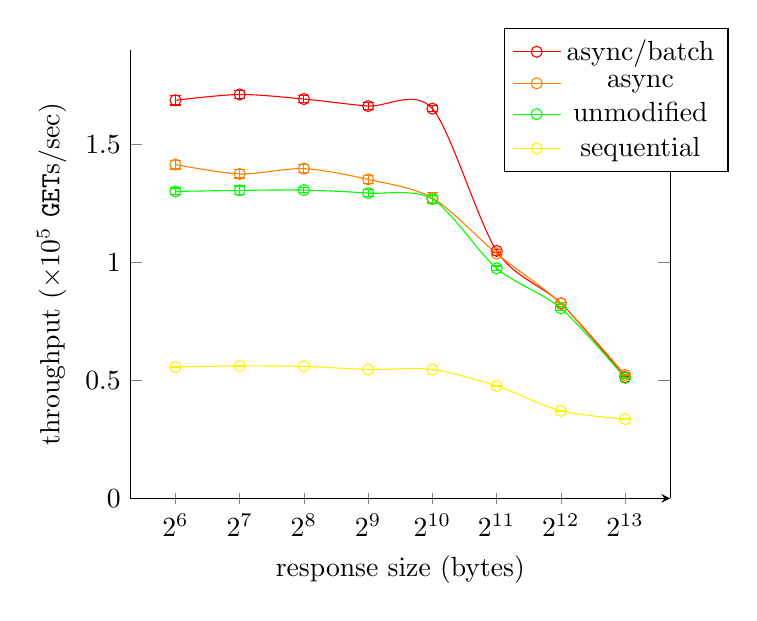
\begin{tikzpicture}
    \begin{axis}[
%        ylabel=throughput (1000 messages/sec),
        xlabel=response size (bytes),
        xmode=log, log basis x=2,
        axis x line=left,
% https://tex.stackexchange.com/questions/351168/pgfplots-get-the-axis-exponent-in-scientific-notation/351349
       ytick scale label code/.code={\pgfmathparse{int(#1)} throughput ($\times 10^{\pgfmathresult}$ \inlinecode{GET}s/sec)},
        every y tick scale label/.style={at={(yticklabel cs:0.5)}, anchor = south, rotate = 90},
        enlarge x limits={0.1},
        legend style={at={(0.9,1.05)},anchor=north},
        ymin=0
    ]
    
    \addplot[
        smooth,
        mark=o,
        red,
        error bars/.cd,
        y dir=both,
        y explicit,
    ] plot coordinates {
        (2^6, 168721.472500) +=(0,1996.924895) -=(0, 1996.924895)
    	(2^7, 171190.161667) +=(0,1528.869557) -=(0, 1528.869557)
    	(2^8, 169241.258333) +=(0,1627.711404) -=(0, 1627.711404)
    	(2^9, 166282.783000) +=(0,1514.494435) -=(0, 1514.494435)
    	(2^10, 165161.173417) +=(0,1339.568466) -=(0, 1339.568466)
    	(2^11, 104904.171667) +=(0,510.922868) -=(0, 510.922868)
    	(2^12, 82667.730750) +=(0,375.841484) -=(0, 375.841484)
    	(2^13, 51389.966667) +=(0,357.138652) -=(0, 357.138652)
    };
    \addlegendentry{async/batch}
    
    \addplot[
        smooth,
        mark=o,
        orange,
        error bars/.cd,
        y dir=both,
        y explicit,
    ] plot coordinates {
    	(2^6, 141489.498917) +=(0,1883.775023) -=(0, 1883.775023)
    	(2^7, 137500.158917) +=(0,1732.652680) -=(0, 1732.652680)
        (2^8, 139735.448917) +=(0,1674.710685) -=(0, 1674.710685)
    	(2^9, 135195.674667) +=(0,1831.268784) -=(0, 1831.268784)
    	(2^10, 127328.943667) +=(0,2149.238820) -=(0, 2149.238820)
    	(2^11, 103748.971250) +=(0,737.150099) -=(0, 737.150099)
    	(2^12, 82599.582500) +=(0,568.180388) -=(0, 568.180388) % RERUN IF YOU HAVE TIME
    	(2^13, 52325.820667) +=(0,242.148297) -=(0, 242.148297)
    };
    \addlegendentry{async}
    
    \addplot[
        smooth,
        mark=o,
        green,
        error bars/.cd,
        y dir=both,
        y explicit,
    ] plot coordinates {
    	(2^6, 130092.183500) +=(0,1466.641377) -=(0, 1466.641377)
    	(2^7, 130525.925333) +=(0,1863.771484) -=(0, 1863.771484)
		(2^8 ,130672.201250) +=(0,1166.766993) -=(0, 1166.766993)
		(2^9 ,129395.225750) +=(0,1536.804499) -=(0, 1536.804499)
		(2^10 ,126869.968750) +=(0,1661.153740) -=(0, 1661.153740)
	    (2^11, 97514.609000) +=(0,961.166348) -=(0, 961.166348)
	    (2^12, 80562.237833) +=(0,845.454959) -=(0, 845.454959)
	    (2^13, 51063.300667) +=(0,365.179556) -=(0, 365.179556)
%	    (2^14, 25045.570917) +=(0,138.171821) -=(0, 138.171821)
    };
    \addlegendentry{unmodified}

    \addplot[
        smooth,
        mark=o,
        yellow,
        error bars/.cd,
        y dir=both,
        y explicit,
    ] plot coordinates {
    	(2^6, 55702.281250) +=(0,71.464026) -=(0, 71.464026)
    	(2^7, 56137.393417) +=(0,77.152816) -=(0, 77.152816)
    	(2^8 ,55941.166083) +=(0,84.756979) -=(0, 84.756979)
    	(2^9, 54658.094000) +=(0,95.221322) -=(0, 95.221322)
    	(2^10, 54614.841250) +=(0,75.334475) -=(0, 75.334475)
    	(2^11, 47651.412583) +=(0,249.905014) -=(0, 249.905014)
    	(2^12, 37113.566250) +=(0,123.533401) -=(0, 123.533401)
    	(2^13, 33634.470083) +=(0,58.558777) -=(0, 58.558777)
%    	(2^14, 19134.664917) +=(0,33.150985) -=(0, 33.150985)
    };
    \addlegendentry{sequential}

    
    \end{axis}
\end{tikzpicture}
\caption{Throughputs of Redis server variants with 95\% confidence intervals.}
\label{fig:main}
\end{figure}


%In this section, I present and analyze the results of my experiments.
%I elaborate on how the results of each benchmark can be used to understand the throughput of the Redis server that has been augmented to use io\_uring to perform batched, asynchronous writes.
The results of the evaluation can be seen in Figure \ref{fig:main}.
It shows the maximum throughput of each variant of the Redis server for a variety of response sizes: the unmodified server, the async/batch server, the async server, and the sequential server.
All means are presented with 95\% confidence intervals, but the size of the confidence interval makes them difficult to see.

All variants of the Redis server outperform the sequential server, which submits each write to a client's socket to \inlinecode{io\_uring} and then waits for completion.
%This can be explained by the fact that the Redis server natively uses socket multiplexing (e.g., select, epoll, kqueue) to determine when a client socket is writable.
%It then uses non-blocking I/O to perform that write \cite{redis-client}.
%The Redis server uses a single thread of execution.
This can likely be attributed to the overhead in putting the writing thread to sleep after submitting the write to \inlinecode{io\_uring} and waking the thread up once the write has been completed.

The async server outperforms the unmodified server by up to 8.7\% for responses of size $2^{6}$ to $2^{9}$ bytes.
The difference in throughput can be understood as the gains made from executing write calls asynchronously via \inlinecode{io\_uring}.
For responses of size $2^{10}$ to $2^{13}$ bytes, both systems have throughput that is on par.

%unmodified server performs on par with the asynchronous io\_uring Redis server, which was adapted to immediately submit each write to a client socket to the io\_uring subsystem for asynchronous execution.
%The Redis server's use of socket multiplexing and non-blocking I/O additionally helps explain the similarity in throughput.
%It suggests that the throughput gains of asynchronous writes compared to performing non-blocking writes are lost as a result of io\_uring's implementation or my implementation in submitting the asynchronous write.

The throughput of the async/batch server performs significantly better than both the unmodified and async servers for responses of size $2^{6}$ to $2^{10}$ bytes.
For this range of sizes, the async/batch server outperforms the async server by up to 29\%.
This result can be understood as the gains made from batching writes to client sockets and thereby reducing system calls.
Additionally, this server outperforms the unmodified server by up to 31\%.
This result can be understood as the gains made from executing batched writes to client sockets asynchronously using \inlinecode{io\_uring}.
Similar to the async server, throughput is on par with the unmodified server for response sizes of $2^{11}$ to $2^{13}$ bytes.

For larger response sizes, throughput is similar for the unmodified, async, and async/batch servers.
%This may be explained by the Redis server spending more time reading from client sockets, resulting in ...

\begin{figure}[h!]
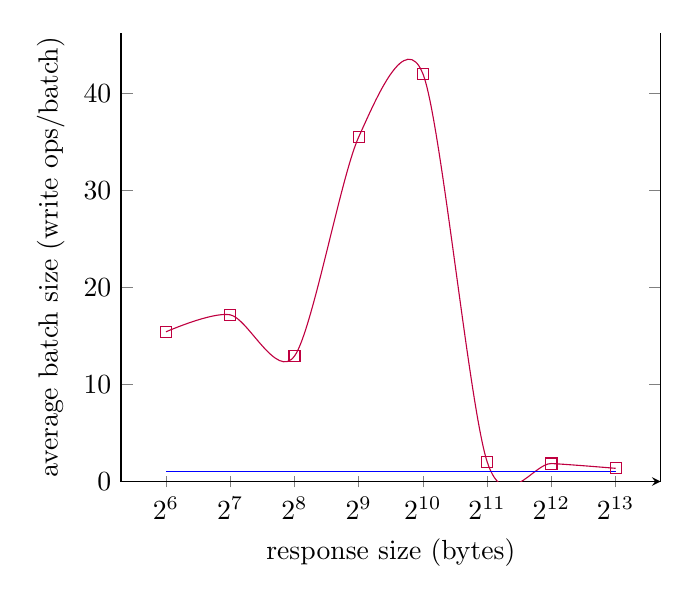
\begin{tikzpicture}
    \begin{axis}[
        ylabel=average batch size (write ops/batch),
        xlabel=response size (bytes),
        xmode=log, log basis x=2,
        axis x line=left,
        enlarge x limits={0.1},
        ymin=0
    ]
    
    \addplot[
        smooth,
        mark=square,
        purple,
        error bars/.cd,
        y dir=both,
        y explicit,
    ] plot coordinates {
        (2^6, 15.41770339280496746486)
        (2^7, 17.16826010747374481793)
        (2^8, 12.91911871627490204246)
        (2^9, 35.48837689390900679748)
        (2^10, 41.97185498620342460952)
        (2^11, 2.01538723069613005865)
        (2^12, 1.85118376652192420188)
        (2^13, 1.35984650337627150376)
    };
    
    \addplot[color=blue] coordinates {(2^6,1) (2^13,1)};

    \end{axis}
\end{tikzpicture}
\caption{Average number of write operations to client sockets batched into a call to \inlinecode{io\_uring\_enter} by the async/batch Redis server.}
\label{fig:writes_per_batch}
\end{figure}

Figure \ref{fig:writes_per_batch} shows the average number of write operations to client sockets submitted to \inlinecode{io\_uring} with a single call to \inlinecode{io\_uring\_enter} by the async/batch server.
The average number of batched writes starts off around 15 writes per batch for responses of size $2^6$ to $2^8$ bytes.
It then rapidly increases to about 35 for $2^9$ bytes and increases again to nearly 42 for $2^{10}$ bytes.
Finally, it drops and plateaus at nearly 1.5 for responses of size $2^{11}$ to $2^{13}$ bytes.
This has been made more clear by a blue line at $y=1$.

These results help explain the similarity of the async/batch server's throughput as compared with that of the async server for the larger response sizes.
The async server can be understood as the async/batch server but with a batch size always equal to one.
Further, these results suggest that better performance can be achieved by controlling the number of entries submitted in each call to \inlinecode{io\_uring\_enter}.

\subsection{Pipelining}
In order to better understand how the Redis server might be affected by performing asynchronous, batched writes to client sockets, the performance of the async/batch server that has been further augmented to support pipelining of commands is evaluated.
Redis uses a Request/Response protocol~\cite{redis-pipeline}.
This means that, after a given client has submitted a request to the server, it must wait for a response prior to submitting another request.
With pipelining, the client can submit several requests at once without waiting for the server to respond.
The server will send responses in the order that the client submits the requests.

\begin{figure}[]
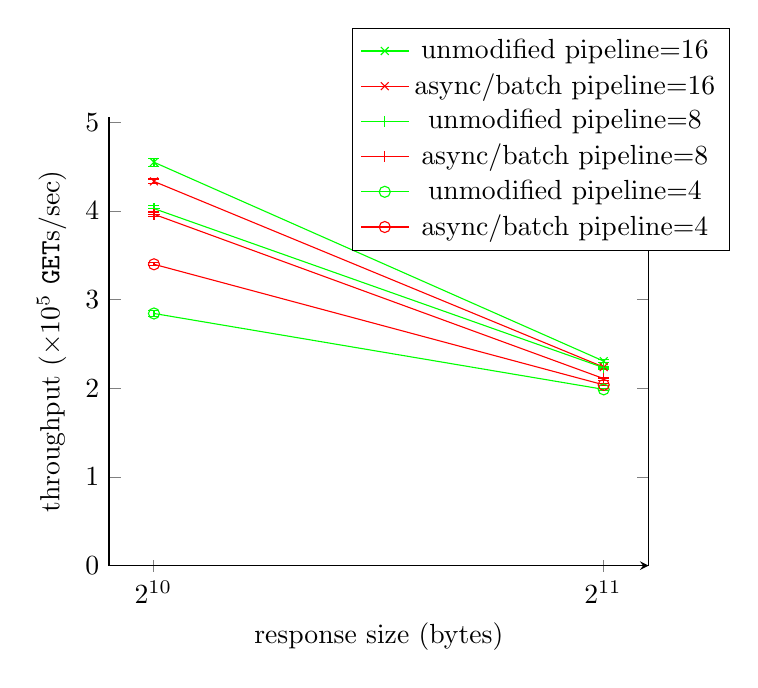
\begin{tikzpicture}
    \begin{axis}[
%        ylabel=throughput (1000 messages/sec),
        xlabel=response size (bytes),
        xmode=log, log basis x=2,
        axis x line=left,
% https://tex.stackexchange.com/questions/351168/pgfplots-get-the-axis-exponent-in-scientific-notation/351349
       ytick scale label code/.code={\pgfmathparse{int(#1)} throughput ($\times 10^{\pgfmathresult}$ \inlinecode{GET}s/sec)},
        every y tick scale label/.style={at={(yticklabel cs:0.5)}, anchor = south, rotate = 90},
        enlarge x limits={0.1},
        legend style={at={(0.8,1.2)},anchor=north},
        ymin=0
    ]
    
    \addplot[
        smooth,
        mark=x,
        green,
        error bars/.cd,
        y dir=both,
        y explicit,
    ] plot coordinates {
    	(2^10, 454875.517750) +=(0,4660.870601) -=(0, 4660.870601)
		(2^11, 230574.502833) +=(0,1795.985333) -=(0, 1795.985333)
    };
    \addlegendentry{unmodified pipeline=16}
    
    \addplot[
        smooth,
        mark=x,
        red,
        error bars/.cd,
        y dir=both,
        y explicit,
    ] plot coordinates {
    	(2^10, 433216.428083) +=(0,2730.896675) -=(0, 2730.896675)
    	(2^11, 223855.657667) +=(0,994.223240) -=(0, 994.223240)
    };
    \addlegendentry{async/batch pipeline=16}

    \addplot[
        smooth,
        mark=+,
        green,
        error bars/.cd,
        y dir=both,
        y explicit,
    ] plot coordinates {
    	(2^10, 402582.520583) +=(0,3983.138266) -=(0, 3983.138266)
    	(2^11, 223209.374833) +=(0,1418.246954) -=(0, 1418.246954)
    };
    \addlegendentry{unmodified pipeline=8}
    
    \addplot[
        smooth,
        mark=+,
        red,
        error bars/.cd,
        y dir=both,
        y explicit,
    ] plot coordinates {
    	(2^10, 396208.634833) +=(0,2543.084697) -=(0, 2543.084697)
    	(2^11, 210889.928083) +=(0,1655.255220) -=(0, 1655.255220)
    };
    \addlegendentry{async/batch pipeline=8}

    \addplot[
        smooth,
        mark=o,
        green,
        error bars/.cd,
        y dir=both,
        y explicit,
    ] plot coordinates {
    	(2^10, 284334.707083) +=(0,3543.712490) -=(0, 3543.712490)
        (2^11, 198761.798833) +=(0,1319.611817) -=(0, 1319.611817)
    };
    \addlegendentry{unmodified pipeline=4}
    
    \addplot[
        smooth,
        mark=o,
        red,
        error bars/.cd,
        y dir=both,
        y explicit,
    ] plot coordinates {
    	(2^10, 339789.081750) +=(0,1594.473770) -=(0, 1594.473770)
    	(2^11, 203868.265000) +=(0,1087.206746) -=(0, 1087.206746)
    };
    \addlegendentry{async/batch pipeline=4}
    
    \end{axis}
\end{tikzpicture}
\caption{Average number of writes to client sockets submitted to kernel using a single \inlinecode{io\_uring\_enter} system call by the Redis server.}
\label{fig:pipelining}
\end{figure}

Enforcing this ordering constraint becomes a challenge when sending responses to clients asynchronously.
In order to support pipelining, writes to a given client socket submitted to \inlinecode{io\_uring} in a given batch and in different batches must be executed in order.

\inlinecode{io\_uring} enables this to be done using the \inlinecode{IOSQE\_IO\_LINK} and \inlinecode{IOSQE\_IO\_DRAIN} flags for the submission queue entries~\cite{iouring}.
The \inlinecode{IOSQE\_IO\_LINK} flag signals that a submission queue entry is a link in a chain.
All sequential submission queue entries with this flag set and the following entry constitute a chain.
A chain is executed in order from head to tail.
This flag is used to ensure that writes to a given client's socket submitted in a single batch are executed in order.
The \inlinecode{IOSQE\_IO\_DRAIN} flag signals that all submission queue entries ahead of the current entry in the queue must be completed before any entries behind the current can begin being executed.
This flag is used to ensure that writes to a given client's socket submitted in different batches are executed in order.

The throughput of the unmodified and async/batch servers are presented in Figure \ref{fig:pipelining} for a variety of response sizes and pipeline depths.
%Figure \ref{fig:pipelining} was generated by performing the above described augmentation to the batching io\_uring Redis server in order for it to support pipelining.
%The system was evaluated using server response sizes of $2^{10}$ and $2^{11}$ bytes.
%Pipeline depth was varied between four, eight, and sixteen commands.

With a pipeline depth of four, the async/batch server's throughput is over 19\% higher than that of the unmodified server for a response size $2^{10}$ bytes.
When the pipeline depth is eight, both servers have approximately the same performance.
Finally, when the pipeline depth is sixteen, the async/batch server has throughput nearly 5\% lower than that of the unmodified server.
These results suggest that \inlinecode{io\_uring} alone should not be used to enforce ordering of write operations to a given client's socket.
The server might have better performance if it enforces ordering of these asynchronous writes by selectively submitting write operations to \inlinecode{io\_uring}.

%\inlinecode{IOSQE\_IO\_LINK} and \inlinecode{IOSQE\_IO\_DRAIN} flags to enforce server response ordering is not scalable.
%Further, in order to enforce such an ordering, the server will need to enforce this ordering by determining when to submit operations to io\_uring.

For any of the given pipeline depths, both servers perform on par with response sizes of $2^{11}$ bytes.
This is the same phenomenon observed in Figure \ref{fig:main}.


\section{Future Work}
In the implementation, writes are submitted to the \inlinecode{io\_uring} framework every cycle around the server's main loop.
This results in batch sizes being largely left to chance.
Considering the results presented in this paper, a next step in this work is to evaluate the performance when submitting batches at regular intervals or after some threshold batch size has been reached.
Additionally, batching will likely result in higher latencies and it would be interesting to investigate how batching affects these values.

In the implementation, the Redis server was not adapted to read from client sockets using \inlinecode{io\_uring}.
The challenge in performing asynchronous reads of client sockets using \inlinecode{io\_uring} is in determining where to store the read data.
When a given client's socket is ready to be read from, the Redis server reserves space on a buffer owned by the client and reads as much data as will fit in the reserved space.
Performing this using \inlinecode{io\_uring} first requires allocating a buffer with specific alignment constraints.
Then, a read operation of the client's socket must be submitted to 
\inlinecode{io\_uring} such that the result is written to the previously allocated buffer.
This operation should be submitted prior to the point at which the client's socket becomes readable.
Once the read has occurred, the server must then wait until it can retrieve the read data from the \inlinecode{io\_uring} completion queue.
For efficiency, the server might want to keep a linked list of buffers per client in order to avoid copying the data to a different location.

\section{Conclusion}
In this work, the Redis server is adapted to make use of Linux's \inlinecode{io\_uring} framework in order to write responses to Redis clients.
Through this adaptation, the performance benefits that can be gained using asynchronous writes to client sockets with fewer system calls are examined.
It is shown that, by using \inlinecode{io\_uring}, the maximum throughput of the Redis server can be increased by as much as 31\% as compared to the unmodified Redis server.
This work demonstrates what performance gains can be achieved using the \inlinecode{io\_uring} framework in a high performance, system intensive scenario.


\section{Acknowledgments}
I would like to acknowledge Professor Benard Wong, who provided me much help and encouragement.


\section{Availability}
Server code can be found \href{https://github.com/bryantcurto/redis/compare/6.0...iouring}{(here)} and benchmarking code can be found \href{https://github.com/bryantcurto/redis/compare/6.0...test-iouring}{(here)}.

%{\footnotesize \bibliographystyle{acm} \bibliography{references.bib}}

\bibliographystyle{ACM-Reference-Format}
\bibliography{references}

\end{document}